%!TEX TS-program = xelatex
\documentclass[]{friggeri-cv}
\usepackage{afterpage}
\usepackage{hyperref}
\usepackage{color}
\usepackage{xcolor}
\usepackage{smartdiagram}

\usepackage{fontspec}
% if you want to add fontawesome package
% you need to compile the tex file with LuaLaTeX
% References:
%   http://texdoc.net/texmf-dist/doc/latex/fontawesome/fontawesome.pdf
%   https://www.ctan.org/tex-archive/fonts/fontawesome?lang=en
%\usepackage{fontawesome}
\usepackage{metalogo}
\usepackage{dtklogos}
\usepackage[utf8]{inputenc}
\usepackage{tikz}
\usetikzlibrary{mindmap,shadows}
\hypersetup{
    pdftitle={},
    pdfauthor={},
    pdfsubject={},
    pdfkeywords={},
    colorlinks=false,           % no lik border color
    allbordercolors=white       % white border color for all
}

\smartdiagramset{
    bubble center node font = \footnotesize,
    bubble node font = \footnotesize,
    % specifies the minimum size of the bubble center node
    bubble center node size = 0.5cm,
    %  specifies the minimum size of the bubbles
    bubble node size = 0.5cm,
    % specifies which is the distance among the bubble center node and the other bubbles
    distance center/other bubbles = 0.3cm,
    % sets the distance from the text to the border of the bubble center node
    distance text center bubble = 0.5cm,
    % set center bubble color
    bubble center node color = pgray,
    % define the list of colors usable in the diagram
    set color list = {lightgray, materialcyan, orange, green, materialorange, materialteal, materialamber, materialindigo, materialgreen, materiallime},
    % sets the opacity at which the bubbles are shown
    bubble fill opacity = 0.6,
    % sets the opacity at which the bubble text is shown
    bubble text opacity = 0.5,
}

%\addbibresource{bibliography.bib}
\RequirePackage{xcolor}
\definecolor{pblue}{HTML}{0395DE}
\definecolor{pgray}{HTML}{6E6E6E}

\begin{document}
\header{\hspace{1.2cm}Aaron David}{ Schneider}{astrophysicist}


% Fake text to add separator
\fcolorbox{white}{gray}{\parbox{\dimexpr\textwidth-2\fboxsep-2\fboxrule}{%
.....
}}

% In the aside, each new line forces a line break
\begin{aside}
  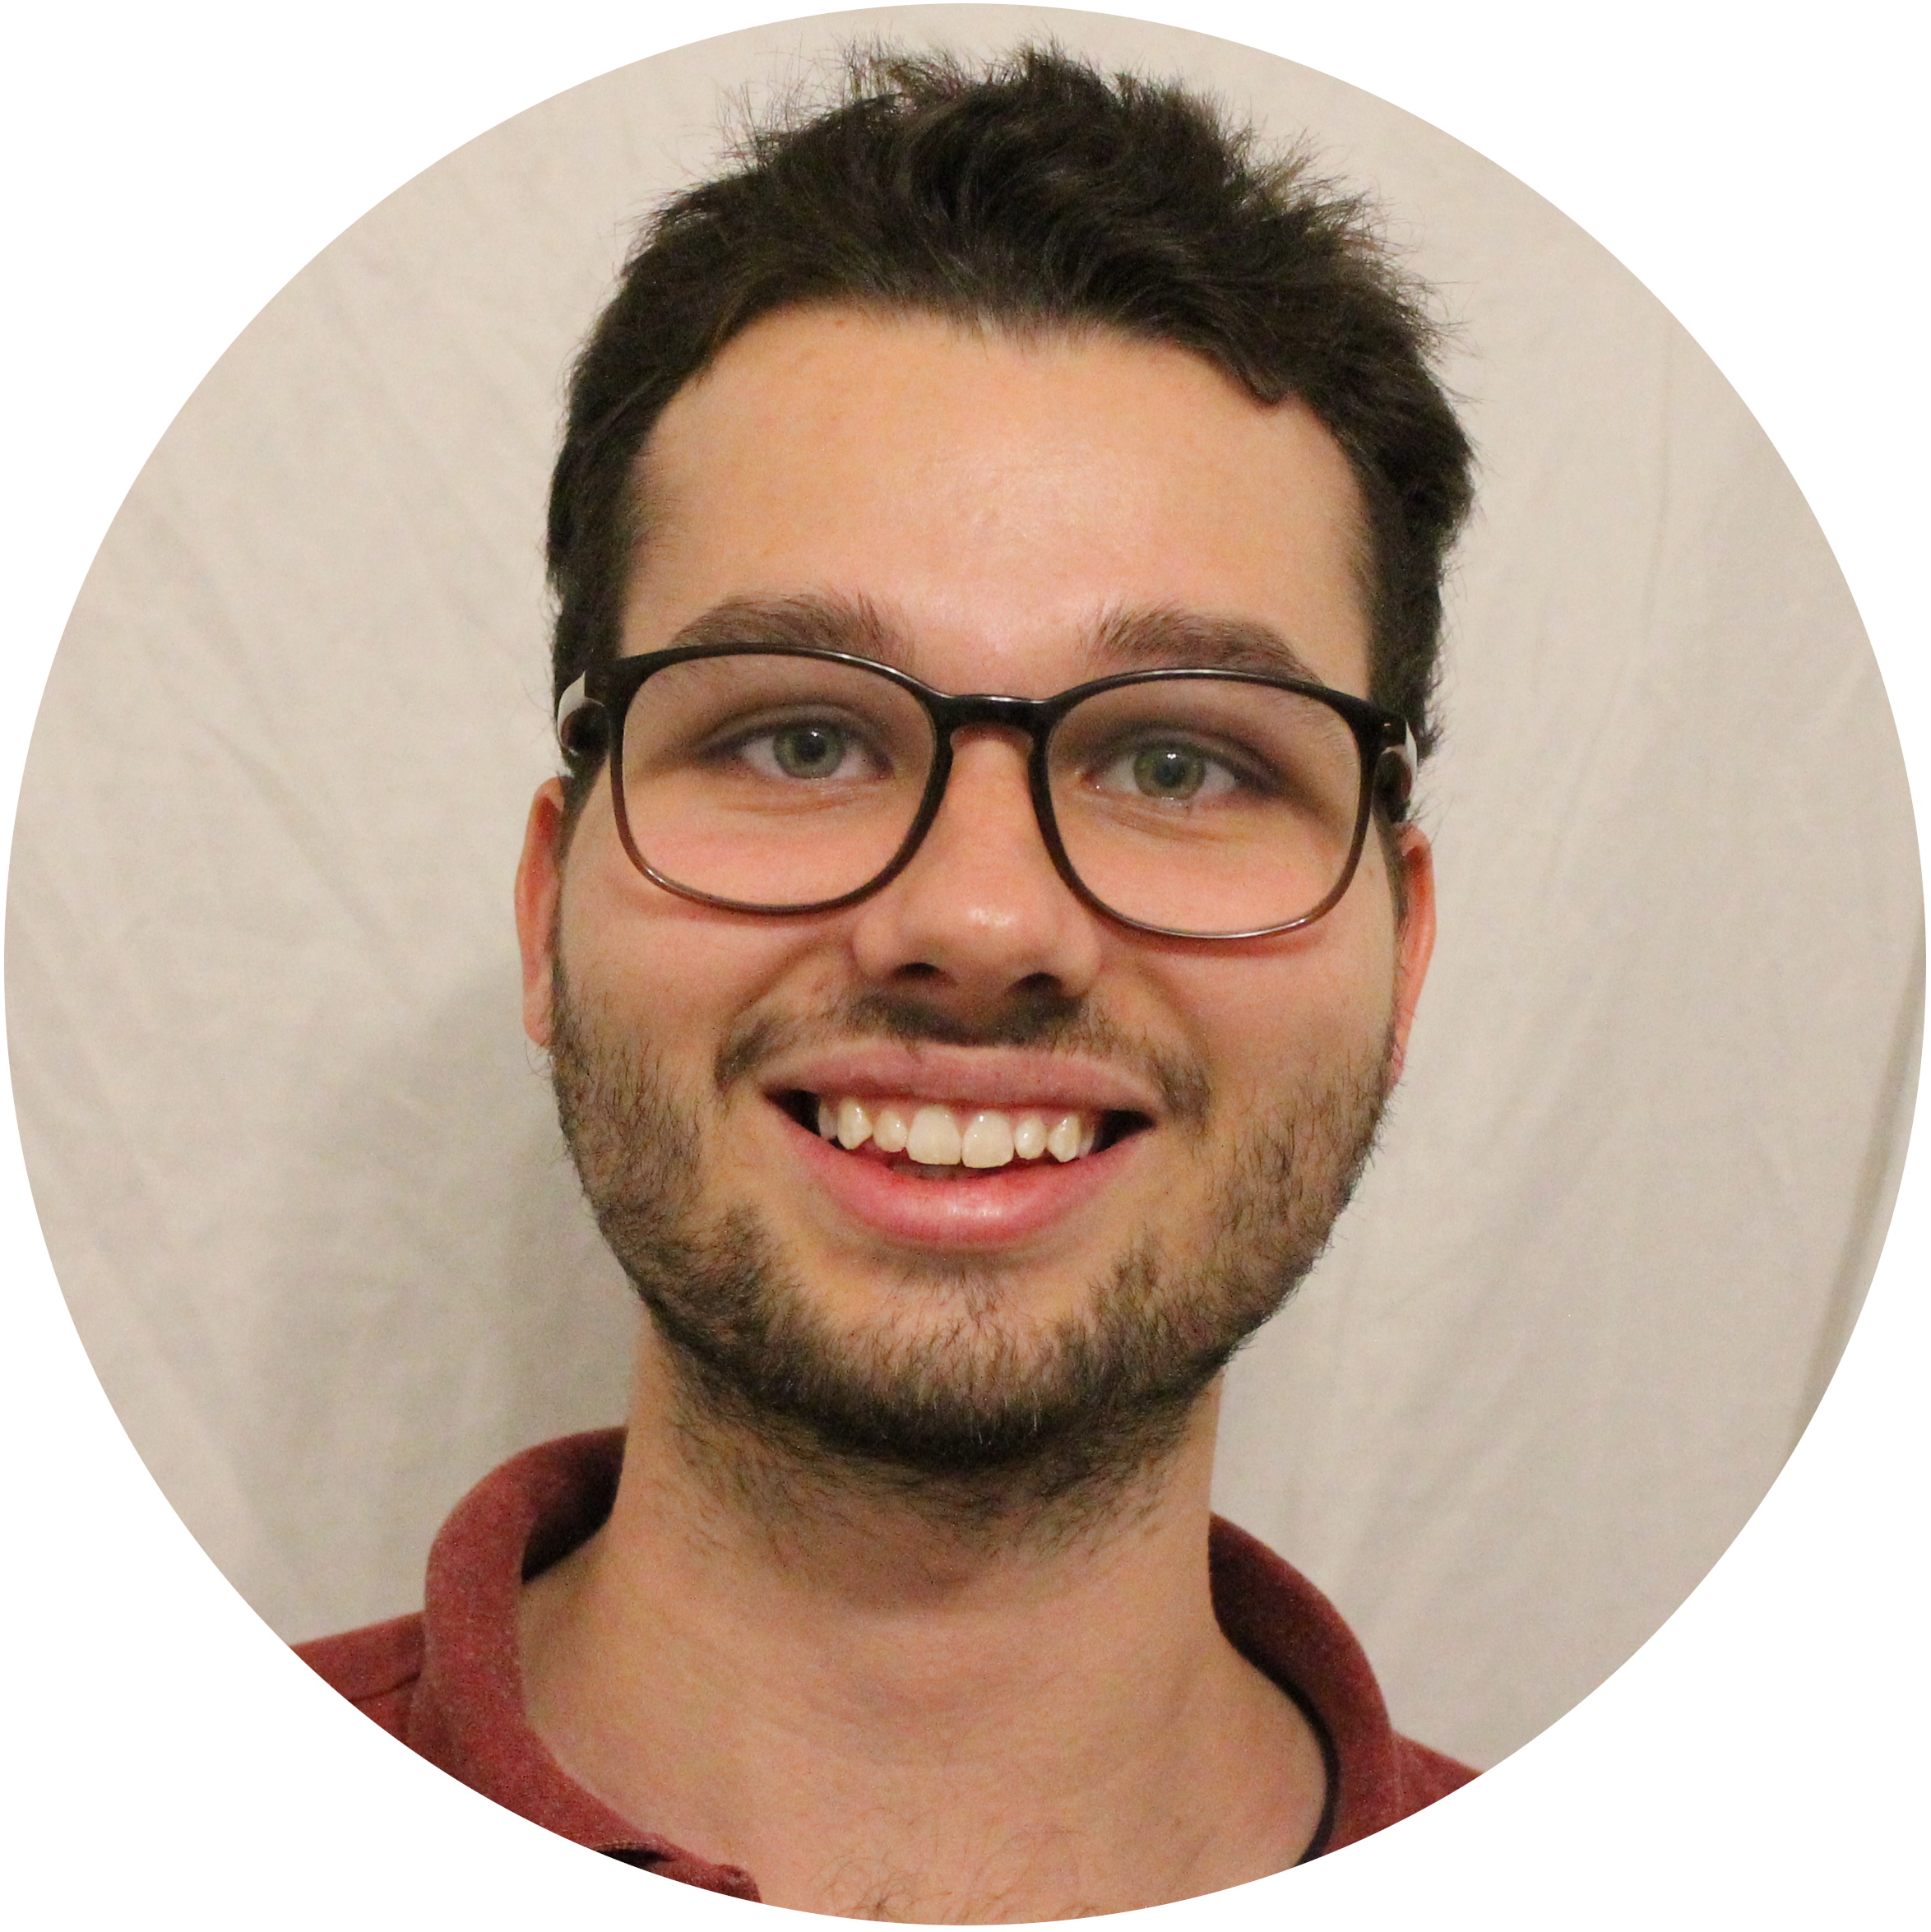
\includegraphics[scale=0.04]{img/Aaron_Circle}
\section{Contact}
~
\textbf{address}
   Rosenweg 10-12
   69221 Dossenheim
   ~
 \textbf{mobile}
 +49 178 316 1990
 ~
 \textbf{mail}
   \href{mailto:aaron@schneiders-hd.de}{\textbf{aaron@}\\schneiders-hd.de}
\section{About Me}
~  
\textbf{nationality}
  german
   ~
  \textbf{birthplace}
  Siegen, Germany
  ~
  \textbf{civil status}
  married
  \section{Programming}
    \smartdiagram[bubble diagram]{
        \textbf{Python},
        \textbf{C/C++\vspace{0.5cm}},
        \textbf{CUDA\vspace{0.5cm}},
        \textbf{LaTeX\vspace{0.5cm}},
        \textbf{Bash\vspace{0.5cm}},
        \textbf{Other}
    }
    \textbf{github:} 
    \href{https://github.com/AaronDavidSchneider/}{@AaronDavidSchneider}
     \section{Languages}
	  ~
    \textbf{german}
    first language
    ~
    \textbf{english}
    fluent
 \section{Interests}
~
 hiking
 singing
  road racing
   programming
\end{aside}

\section{Education}
\begin{entrylist}
  \entry
    {10/15-08/18}
    {Bachelor in Physics}
    {Universität Heidelberg}
    {\begin{itemize}\vspace{-3mm}
    	\item grade: 2.0 (UK: B)
    	\item specialization: astrophysics and computational physics
    	\item bachelor thesis: Surface waves in protoplanetary disks induced by outbursts
    	\item supervisor of thesis: Prof.Dr. Cornelis P. Dullemond
    \end{itemize}
	}
	\\
  \entry
    {10/18-10/20}
    {Master in Physics}
    {Universität Heidelberg}
    {\begin{itemize}\vspace{-3mm}
    	\item expected grade: $~$1.5 (UK: A)
    	\item specialization: Machine Learning and GPU Computing
    	\item core courses: astronomical techniques, general relativity, theoretical astrophysics, cosmology, environomental physics
    	\item master thesis: chemical composition of gas giants probed by accretion
    	\item supervisor of thesis: Dr. Bertram Bitsch
    \end{itemize}
	}
\end{entrylist}
\section{Schooling}
\begin{entrylist}
  \entry
    {09/06-06/14}
    {Highschool}
    {Evangelisches Gymnasium Siegen-Weidenau}
    {\begin{itemize}\vspace{-3mm}
		\item advanced courses: physics, math
		\item A-level: Grade 1.6 (UK: A)
	\end{itemize}}
\end{entrylist}
\section{Experience}
\begin{entrylist}
	\entry
    {09/14-06/15}
    {year abroad}
    {Carnforth, England}
    {theology studies}
	\entry
    {since 2016}
    {private tutition}
    {Heidelberg}
    {highschool math and physics}

\end{entrylist}
\section{Publications}
\begin{entrylist}
  \entry
    {09/18}
    {A \& A, Volume 617, id.L7}
    {Schneider, A. D.; Dullemond, C. P.; Bitsch, B.}
    {Surface waves in protoplanetary disks induced by outbursts: Concentric rings in scattered light}
\end{entrylist}
\section{Volunteer Engagement}
\begin{entrylist}
  \entry
    {2015-2019}
    {voluntary work at a christian university group}
    {Heidelberg}
    {Hochschul SMD Heidelberg}
\end{entrylist}
\vspace{1.3cm}
\begin{flushright}

\includegraphics[width=.2\textwidth]{img/signature}\\
\emph{Aaron David Schneider, November 18th, 2019}
\end{flushright}
\clearpage

%\section{Publications}
%Author, Author, Author\\
%\textbf{Lorem ipsum dolor sit amet, consectetur adipiscing elit, sed do eiusmod tempor incididunt ut labore et dolore magna aliqua}\\
%\emph{Lorem ipsum dolor sit amet, consectetur adipiscing elit, sed do eiusmod tempor incididunt ut labore et dolore magna aliqua}
%\\
%\section{Honors \& Awards}
%\begin{entrylist}
%  \entry
%    {10/2015}
%    {Best swordsman duel}
%    {Contest}
%    {Lorem ipsum.\\
%    \emph{Lorem ipsum}}
%\end{entrylist}
%
%\section{Certifications}
%\begin{entrylist}
%  \entry
%    {02/2013}
%    {Intro to Computer Science}
%    {Udacity. E-learning}
%    {\emph{Building a Python Search Engine}}
%\end{entrylist}
%
%\section{Other Info}
%For the Italian job market:\\
%\emph{Si autorizza il trattamento delle informazioni contenute nel curriculum in conformità alle disposizioni previste dal d.lgs. 196/2003. Si dichiara altresì di essere consapevole che, in caso di dichiarazioni non veritiere, si è passibili di sanzioni penali ai sensi del DPR 445/00 oltre alla revoca dei benefici eventualmente percepiti.}
%\\
%\begin{flushleft}
%\emph{May 8th, 2016}
%\end{flushleft}
%\begin{flushright}
%\emph{John Snow}
%\end{flushright}
\end{document}